\documentclass{standalone}
\usepackage{tikz}
\usetikzlibrary{patterns, positioning}

\begin{document}
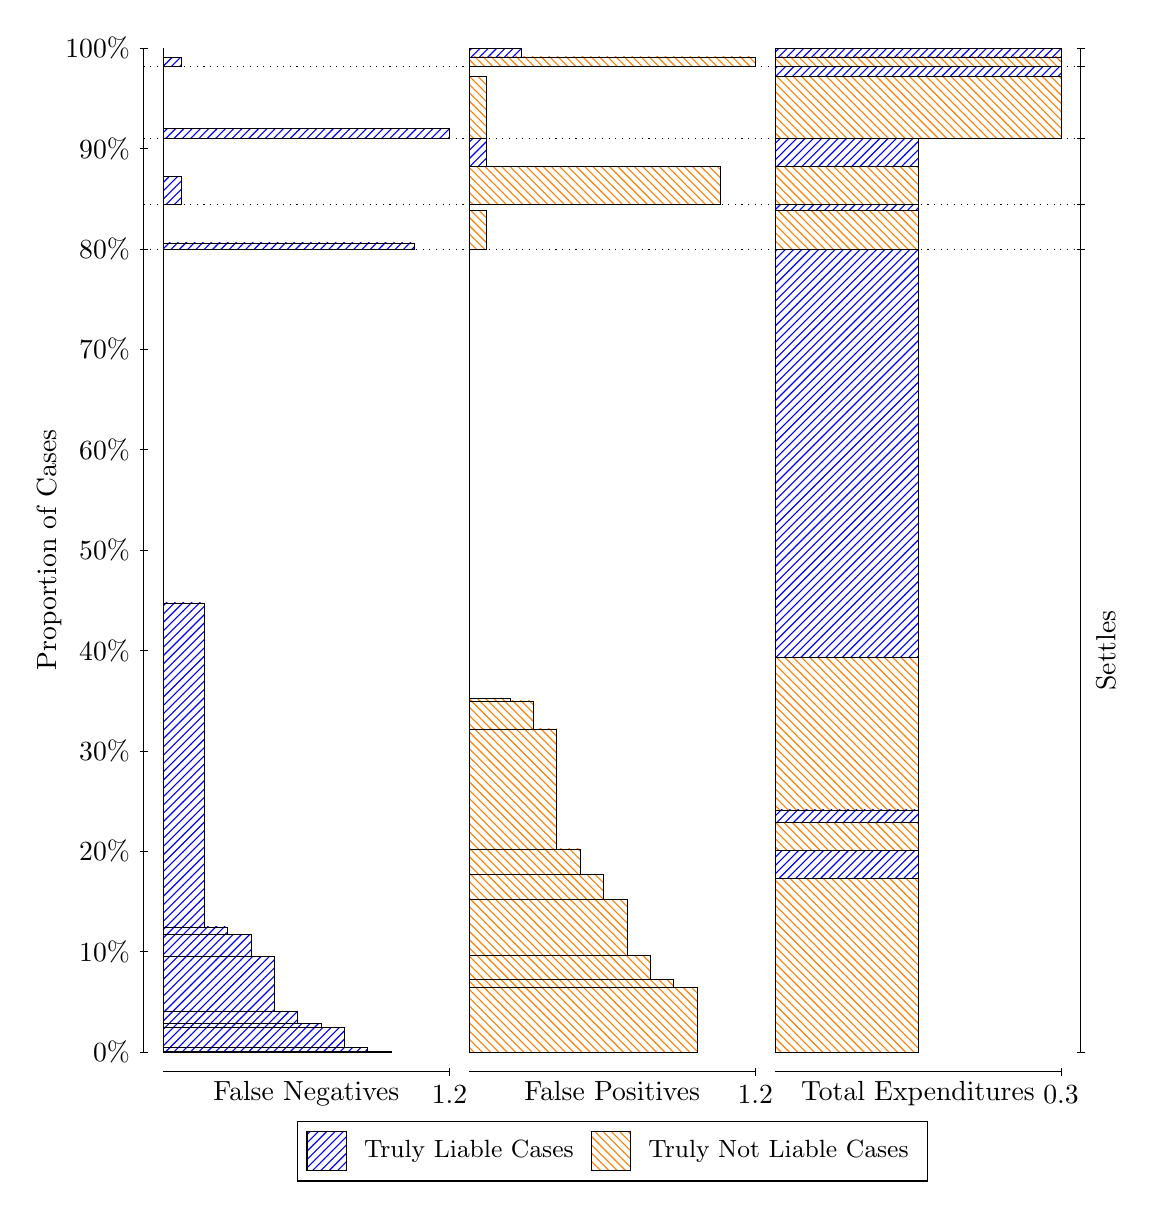
\begin{tikzpicture}
\draw[black, very thin] (1.5,1.75) -- (1.5,14.5);
\node[rotate=90, anchor=center] at (0.3, 8.125) {Proportion of Cases};
\draw[black, very thin] (1.45,1.75) -- (1.55,1.75);
\node[anchor=east] at (1.45, 1.75) {0\%};
\draw[black, very thin] (1.45,3.025) -- (1.55,3.025);
\node[anchor=east] at (1.45, 3.025) {10\%};
\draw[black, very thin] (1.45,4.3) -- (1.55,4.3);
\node[anchor=east] at (1.45, 4.3) {20\%};
\draw[black, very thin] (1.45,5.575) -- (1.55,5.575);
\node[anchor=east] at (1.45, 5.575) {30\%};
\draw[black, very thin] (1.45,6.85) -- (1.55,6.85);
\node[anchor=east] at (1.45, 6.85) {40\%};
\draw[black, very thin] (1.45,8.125) -- (1.55,8.125);
\node[anchor=east] at (1.45, 8.125) {50\%};
\draw[black, very thin] (1.45,9.4) -- (1.55,9.4);
\node[anchor=east] at (1.45, 9.4) {60\%};
\draw[black, very thin] (1.45,10.675) -- (1.55,10.675);
\node[anchor=east] at (1.45, 10.675) {70\%};
\draw[black, very thin] (1.45,11.95) -- (1.55,11.95);
\node[anchor=east] at (1.45, 11.95) {80\%};
\draw[black, very thin] (1.45,13.225) -- (1.55,13.225);
\node[anchor=east] at (1.45, 13.225) {90\%};
\draw[black, very thin] (1.45,14.5) -- (1.55,14.5);
\node[anchor=east] at (1.45, 14.5) {100\%};

\draw[black, very thin] (13.4,1.75) -- (13.4,14.5);
\draw[black, very thin] (13.35,1.75) -- (13.45,1.75);
\node[anchor=west] at (13.35, 1.75) {};
\draw[black, very thin] (13.35,11.945) -- (13.45,11.945);
\node[anchor=west] at (13.35, 11.945) {};
\draw[black, very thin] (13.35,12.514) -- (13.45,12.514);
\node[anchor=west] at (13.35, 12.514) {};
\draw[black, very thin] (13.35,13.351) -- (13.45,13.351);
\node[anchor=west] at (13.35, 13.351) {};
\draw[black, very thin] (13.35,14.265) -- (13.45,14.265);
\node[anchor=west] at (13.35, 14.265) {};
\draw[black, very thin] (13.35,14.5) -- (13.45,14.5);
\node[anchor=west] at (13.35, 14.5) {};

\draw[black, very thin, pattern color=blue, pattern=north east lines] (1.75,1.75) rectangle (4.6418,1.7555);
\draw[black, very thin, pattern color=blue, pattern=north east lines] (1.75,1.7555) rectangle (4.3452,1.806);
\draw[black, very thin, pattern color=blue, pattern=north east lines] (1.75,1.806) rectangle (4.0486,2.058);
\draw[black, very thin, pattern color=blue, pattern=north east lines] (1.75,2.058) rectangle (3.752,2.1153);
\draw[black, very thin, pattern color=blue, pattern=north east lines] (1.75,2.1153) rectangle (3.4554,2.2672);
\draw[black, very thin, pattern color=blue, pattern=north east lines] (1.75,2.2672) rectangle (3.1588,2.9609);
\draw[black, very thin, pattern color=blue, pattern=north east lines] (1.75,2.9609) rectangle (2.8622,3.2456);
\draw[black, very thin, pattern color=blue, pattern=north east lines] (1.75,3.2456) rectangle (2.5656,3.3378);
\draw[black, very thin, pattern color=blue, pattern=north east lines] (1.75,3.3378) rectangle (2.269,7.4538);
\draw[black, very thin, pattern color=orange, pattern=north west lines] (1.75,7.4538) rectangle (1.75,11.945);
\draw[black, very thin, pattern color=blue, pattern=north east lines] (1.75,11.945) rectangle (4.9384,12.025);
\draw[black, very thin, pattern color=orange, pattern=north west lines] (1.75,12.025) rectangle (1.75,12.514);
\draw[black, very thin, pattern color=blue, pattern=north east lines] (1.75,12.514) rectangle (1.9724,12.867);
\draw[black, very thin, pattern color=orange, pattern=north west lines] (1.75,12.867) rectangle (1.75,13.351);
\draw[black, very thin, pattern color=blue, pattern=north east lines] (1.75,13.351) rectangle (5.3833,13.477);
\draw[black, very thin, pattern color=orange, pattern=north west lines] (1.75,13.477) rectangle (1.75,14.265);
\draw[black, very thin, pattern color=blue, pattern=north east lines] (1.75,14.265) rectangle (1.9724,14.378);
\draw[black, very thin, pattern color=orange, pattern=north west lines] (1.75,14.378) rectangle (1.75,14.5);
\draw[black, very thin, pattern color=orange, pattern=north west lines] (5.6333,1.75) rectangle (8.5252,2.5672);
\draw[black, very thin, pattern color=orange, pattern=north west lines] (5.6333,2.5672) rectangle (8.2286,2.6742);
\draw[black, very thin, pattern color=orange, pattern=north west lines] (5.6333,2.6742) rectangle (7.932,2.9755);
\draw[black, very thin, pattern color=orange, pattern=north west lines] (5.6333,2.9755) rectangle (7.6354,3.6852);
\draw[black, very thin, pattern color=orange, pattern=north west lines] (5.6333,3.6852) rectangle (7.3388,4.0071);
\draw[black, very thin, pattern color=orange, pattern=north west lines] (5.6333,4.0071) rectangle (7.0422,4.3218);
\draw[black, very thin, pattern color=orange, pattern=north west lines] (5.6333,4.3218) rectangle (7.0422,4.3304);
\draw[black, very thin, pattern color=orange, pattern=north west lines] (5.6333,4.3304) rectangle (6.7456,5.8541);
\draw[black, very thin, pattern color=orange, pattern=north west lines] (5.6333,5.8541) rectangle (6.449,6.2101);
\draw[black, very thin, pattern color=orange, pattern=north west lines] (5.6333,6.2101) rectangle (6.1524,6.2414);
\draw[black, very thin, pattern color=blue, pattern=north east lines] (5.6333,6.2414) rectangle (5.6333,11.945);
\draw[black, very thin, pattern color=orange, pattern=north west lines] (5.6333,11.945) rectangle (5.8558,12.434);
\draw[black, very thin, pattern color=blue, pattern=north east lines] (5.6333,12.434) rectangle (5.6333,12.514);
\draw[black, very thin, pattern color=orange, pattern=north west lines] (5.6333,12.514) rectangle (8.8218,12.998);
\draw[black, very thin, pattern color=blue, pattern=north east lines] (5.6333,12.998) rectangle (5.8558,13.351);
\draw[black, very thin, pattern color=orange, pattern=north west lines] (5.6333,13.351) rectangle (5.8558,14.139);
\draw[black, very thin, pattern color=blue, pattern=north east lines] (5.6333,14.139) rectangle (5.6333,14.265);
\draw[black, very thin, pattern color=orange, pattern=north west lines] (5.6333,14.265) rectangle (9.2667,14.387);
\draw[black, very thin, pattern color=blue, pattern=north east lines] (5.6333,14.387) rectangle (6.3007,14.5);
\draw[black, very thin, pattern color=orange, pattern=north west lines] (9.5167,1.75) rectangle (11.333,3.953);
\draw[black, very thin, pattern color=blue, pattern=north east lines] (9.5167,3.953) rectangle (11.333,4.3128);
\draw[black, very thin, pattern color=orange, pattern=north west lines] (9.5167,4.3128) rectangle (11.333,4.666);
\draw[black, very thin, pattern color=blue, pattern=north east lines] (9.5167,4.666) rectangle (11.333,4.8234);
\draw[black, very thin, pattern color=orange, pattern=north west lines] (9.5167,4.8234) rectangle (11.333,6.7586);
\draw[black, very thin, pattern color=blue, pattern=north east lines] (9.5167,6.7586) rectangle (11.333,11.945);
\draw[black, very thin, pattern color=orange, pattern=north west lines] (9.5167,11.945) rectangle (11.333,12.434);
\draw[black, very thin, pattern color=blue, pattern=north east lines] (9.5167,12.434) rectangle (11.333,12.514);
\draw[black, very thin, pattern color=orange, pattern=north west lines] (9.5167,12.514) rectangle (11.333,12.998);
\draw[black, very thin, pattern color=blue, pattern=north east lines] (9.5167,12.998) rectangle (11.333,13.351);
\draw[black, very thin, pattern color=orange, pattern=north west lines] (9.5167,13.351) rectangle (13.15,14.139);
\draw[black, very thin, pattern color=blue, pattern=north east lines] (9.5167,14.139) rectangle (13.15,14.265);
\draw[black, very thin, pattern color=orange, pattern=north west lines] (9.5167,14.265) rectangle (13.15,14.387);
\draw[black, very thin, pattern color=blue, pattern=north east lines] (9.5167,14.387) rectangle (13.15,14.5);
\draw[black, dotted] (1.5,11.945) -- (13.4,11.945);
\draw[black, dotted] (1.5,12.514) -- (13.4,12.514);
\draw[black, dotted] (1.5,13.351) -- (13.4,13.351);
\draw[black, dotted] (1.5,14.265) -- (13.4,14.265);
\draw[black, very thin] (1.75,1.5) -- (5.3833,1.5);
\node[anchor=north] at (3.5667, 1.5) {False Negatives};
\draw[black, very thin] (5.3833,1.45) -- (5.3833,1.55);
\node[anchor=north] at (5.3833, 1.45) {1.2};

\draw[black, very thin] (5.6333,1.5) -- (9.2667,1.5);
\node[anchor=north] at (7.45, 1.5) {False Positives};
\draw[black, very thin] (9.2667,1.45) -- (9.2667,1.55);
\node[anchor=north] at (9.2667, 1.45) {1.2};

\draw[black, very thin] (9.5167,1.5) -- (13.15,1.5);
\node[anchor=north] at (11.333, 1.5) {Total Expenditures};
\draw[black, very thin] (13.15,1.45) -- (13.15,1.55);
\node[anchor=north] at (13.15, 1.45) {0.3};

\node[black, centered, rotate=90] at (13.72, 6.8476) {Settles};





\draw (7.449999999999999,1.5) node[draw=none] (baseCoordinate) {};
\begin{scope}[align=center]
        \matrix[scale=0.5, draw=black, below=0.5cm of baseCoordinate, nodes={draw}, column sep=0.1cm]{
            \node[rectangle, draw, minimum width=0.5cm, minimum height=0.5cm, pattern=north east lines, pattern color=blue] {}; &
            \node[draw=none, font=\small] (B) {Truly Liable Cases}; &
            \node[rectangle, draw, minimum width=0.5cm, minimum height=0.5cm, pattern=north west lines, pattern color=orange] {}; &
            \node[draw=none, font=\small] (B) {Truly Not Liable Cases}; \\
            };
\end{scope}

\end{tikzpicture}
\end{document}